% This is the Reed College LaTeX thesis template. Most of the work 
% for the document class was done by Sam Noble (SN), as well as this
% template. Later comments etc. by Ben Salzberg (BTS). Additional
% restructuring and APA support by Jess Youngberg (JY).
% Your comments and suggestions are more than welcome; please email
% them to cusf@reed.edu
%
% See http://web.reed.edu/cis/help/latex.html for help. There are a 
% great bunch of help pages there, with notes on
% getting started, bibtex, etc. Go there and read it if you're not
% already familiar with LaTeX.
%
% Any line that starts with a percent symbol is a comment. 
% They won't show up in the document, and are useful for notes 
% to yourself and explaining commands. 
% Commenting also removes a line from the document; 
% very handy for troubleshooting problems. -BTS

% As far as I know, this follows the requirements laid out in 
% the 2002-2003 Senior Handbook. Ask a librarian to check the 
% document before binding. -SN

%%
%% Preamble
%%
% \documentclass{<something>} must begin each LaTeX document
\documentclass[12pt,twoside]{reedthesis}
% Packages are extensions to the basic LaTeX functions. Whatever you
% want to typeset, there is probably a package out there for it.
% Chemistry (chemtex), screenplays, you name it.
% Check out CTAN to see: http://www.ctan.org/
%%
\usepackage{graphicx,latexsym} 
\usepackage{amssymb,amsthm,amsmath}
\usepackage{longtable,booktabs,setspace} 
%\usepackage{chemarr} %% Useful for one reaction arrow, useless if you're not a chem major
\usepackage{url}
\usepackage{natbib}
% \usepackage{times} % other fonts are available like times, bookman, charter, palatino

\newcommand{\eqn}[1]{\begin{equation}#1\end{equation}}
\newcommand{\eq}[1]{\begin{align}#1\end{align}}


\title{Quantum Mechanical Bound States of the Yukawa Potential (or some better title)}
\author{Ellen M. McManis}
% The month and year that you submit your FINAL draft TO THE LIBRARY (May or December)
\date{May 2012}
\division{Mathematics and Natural Sciences}
\advisor{Nelia Mann}
%If you have two advisors for some reason, you can use the following
%\altadvisor{Your Other Advisor}
%%% Remember to use the correct department!
\department{Physics}
% if you're writing a thesis in an interdisciplinary major,
% uncomment the line below and change the text as appropriate.
% check the Senior Handbook if unsure.
%\thedivisionof{The Established Interdisciplinary Committee for}
% if you want the approval page to say "Approved for the Committee",
% uncomment the next line
%\approvedforthe{Committee}

\setlength{\parskip}{0pt}
%%
%% End Preamble
%%
%% The fun begins:
\begin{document}

  \maketitle
  \frontmatter % this stuff will be roman-numbered
  \pagestyle{empty} % this removes page numbers from the frontmatter

% Acknowledgements (Acceptable American spelling) are optional
% So are Acknowledgments (proper English spelling)
    \chapter*{Acknowledgements}
	People. Things. Shep, the dog who is currently keeping me company.

% The preface is optional
% To remove it, comment it out or delete it.
%    \chapter*{Preface}
%	This is an example of a thesis setup to use the reed thesis document class.

    \tableofcontents
% if you want a list of tables, optional
    \listoftables
% if you want a list of figures, also optional
    \listoffigures

% The abstract is not required if you're writing a creative thesis (but aren't they all?)
% If your abstract is longer than a page, there may be a formatting issue.
    \chapter*{Abstract}
	Math and computers and stuff gave me results!
		
%	\chapter*{Dedication}
%	You can have a dedication here if you wish.

  \mainmatter % here the regular arabic numbering starts
  \pagestyle{fancyplain} % turns page numbering back on

%The \introduction command is provided as a convenience.
%if you want special chapter formatting, you'll probably want to avoid using it altogether

    \chapter*{Introduction}
         \addcontentsline{toc}{chapter}{Introduction}
	\chaptermark{Introduction}
	\markboth{Introduction}{Introduction}
	% The three lines above are to make sure that the headers are right, that the intro gets included in the table of contents, and that it doesn't get numbered 1 so that chapter one is 1.

% Double spacing: if you want to double space, or one and a half 
% space, uncomment one of the following lines. You can go back to 
% single spacing with the \singlespacing command.
% \onehalfspacing
% \doublespacing
The Yukawa potential describes a force mediated by a massive particle. It is %argh fuck this part
\eqn{
V(r) = -\frac{C}{r}e^{-r/l}\mbox{,}
}
where $C$ and $l$ are constants. $C$ sets the strength of the force; $l$ acts as a length scale. The exponential term provides an effective cutoff once $r$ gets much larger than $l$, as the exponential term drops off quite rapidly. We are interested in how the bound states change with these constants. 

The force described by the potential comes from the exchange of virtual particles. The lenth scale, which limits the range at which the force acts, comes about because the virtual particles exchanged have mass. The mass of these particles then generates the length scale:
\eqn{
l = \frac{\hbar}{m_{\pi}c}\mbox{.}
}
The strength of the force $C$ is only known experimentally and depends on the application of the potential. Most commonly, this is the forces between protons and neutrons in an atomic nucleus.

In general, the time-independent Schr\"odinger wave equation for a particle under the influence of some $V(r)$ is
\eqn{
-\frac{\hbar^2}{2\mu}\nabla^2\psi(r,\phi,\theta) + V(r)\psi (r,\phi,\theta) = E \psi(r,\phi,\theta)
\label{eq:TIDSWE-general}
}
In this thesis, we are working with a system of two particles moving under the influence of the Yukawa potential (in the atomic case, this would be a deuterium nucleus). To simplify the system, it makes the most sense to express this in spherical coordinates as a reduced mass orbiting a center of mass. This is the form used for the wave equation above. With the Yukawa potential, this equation cannot be solved analytically. However, we can solve the more simple system described by the potential without the exponential term, that is,
\eqn{
 V(r) = -\frac{C}{r}\mbox{.}
 }
This potential is the same form as the Coulomb potential in the hydrogen atom. With the Coulomb potential, $C = \frac{e^2}{4\pi \epsilon_0}$. While $r << l$, the Yukawa potential should behave similarly to this, because the $-C/r$ term will dominate. Therefore, we will gain some insight on the Yukawa potential by solving the wave equation for this one.
The solution to this wave equation is well known:
\eqn{
\psi_{l, m_l, n} (r, \theta, \phi) = R_{n,l}(r) Y_{l,m_l}(\theta,\phi)\mbox{.}
}
Here, $l$, $m_l$, and $n$ are quantum numbers. The $Y_{l, m_l}$ are the spherical harmonics. As we are currently interested only in spherically symmetric solutions, we can discard these for the moment, leaving us with
\eqn{
\psi_{n, l =0}(r) = R_{n , l= 0}(r) = e^{-C \mu r / n \hbar^2}\left(\frac{C \mu r}{\hbar^2}\right)^{l} G_{n, l = 0}\left(\frac{C \mu r}{\hbar^2}\right)
\label{eq:SWE-coulomb}
}
The $G_{n,l}$ here is related to the Laguerre polynomials:
\eqn{
G_{n,l}\left(\frac{C \mu r}{\hbar^2}\right) = L^{2l + 1 }_{n- l -1} \left(2\frac{C \mu r}{\hbar^2}\right)\mbox{.}
}
The energy for the particle described by this wave function is just a function of $n$ (the radial quantum number), and is equal to
\eqn{
E_n = -\frac{\mu C^2}{2\hbar^2 n^2}\mbox{.}
}
All of these functions can be simplified further by introducing a length scale, 
\eqn{
\alpha = \frac{\hbar^2}{C \mu}\mbox{.}
\label{eq:bohrradius}
}
$\alpha$ is a constant with units of length, defined in terms of the other constants of the problem. In hydrogen, this is the Bohr radius, and reduces to the familiar $a_o = \frac{4\pi \epsilon_0 \hbar^2}{\mu e^2}$. Physically, $\alpha$ is the length scale of exponential term in the ground state of \eqref{eq:SWE-coulomb}. In hydrogen, this determines the size of the smallest electron cloud. As $n$ increases, so do the possible values of $r$, and the particle can be found further and further from the center of mass of the system. This can be seen in figure \ref{fig:hfuncs}, in which $\psi(r)$ is plotted for several values of $n$.
\begin{figure}
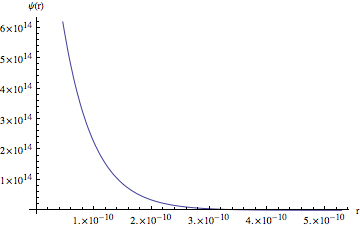
\includegraphics[scale=0.75]{hydground.png}
\caption{The ground state ($n=1$, $l =0$, $m_l= 0$) wave function for hydrogen}
\label{fig:hfuncs}
\end{figure}
As this happens, $E_n$ gets closer and closer to zero, but never quite reaches it -- there are an infinite number of bound states possible. This is shown in figure \ref{fig:hspec}.
\begin{figure}[h]
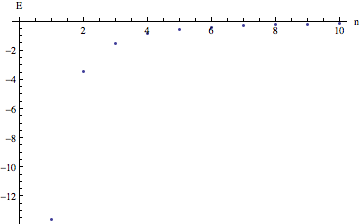
\includegraphics[scale=0.75]{hydrogenspectrum.png}
\caption{The energies of the first 10 bound states of the electron in the hydrogen atom}
\label{fig:hspec}
\end{figure}

Going back to the more-complicated Yukawa potential, the exponential term in the potential means that its range is limited in a way the Coulomb potential's isn't, because $e^{-x}$ drops off much faster than $1/x$. We expect that this will limit the number of bound states as well, to some number whose $r$s are less than $l$.

\clearpage %% starts a new page and stops trying to place floats such as tables and figures

\chapter{Semi-Classical Approximation and Numerical Setup}
\section{The Bohr Model}
The similarity between the Yukawa potential in deuterium and the Coulomb potential in hydrogen suggests treating them similarly. The Bohr model is a semi-classical view of the electron orbiting the nucleus in hydrogen. The postulates of the model are as follows:
\begin{enumerate}
\item Electrons move in circular orbits around the nucleus under the influence of the Coulomb force. They obey all the laws of classical mechanics.
\item Angular momentum is quantized; $L = n\hbar$ where $n$ is a positive integer.
\item The energy of the electron in an orbit remains constant.
\item If an electron changes orbits, electromagnetic radiation is emitted with frequency $\nu = \frac{E_i-E_f}{h}$
\end{enumerate}
We can easily use this model with the Yukawa potential instead of the Coulomb to get a qualitative idea of where we expect bound states to be found.

First, we look at the classical energy of a particle (here, the reduced mass of the neutron-proton system) moving under the influence of the Yukawa potential:
\eqn{
E = \frac{1}{2}\mu \dot{r}^2+\frac{1}{2}\frac{L^2}{\mu r^2}-\frac{C}{r}e^{-r/l}\mbox{.}
\label{eq:classical-energy}
}
To make this easier to work with, we use the length scale from \eqref{eq:bohrradius}, the ``Bohr radius'' for this problem. We then use this to nondimensionalize $r$, defining
\begin{equation}
\rho \equiv \frac{r}{\alpha}\mbox{.}
\label{eq:rho}
\end{equation}
Finally, we define a time scale:
\begin{equation}
\beta \equiv \frac{c^2m}{\hbar^3}\mbox{.}
\label{eq:beta}
\end{equation}

We can now substitute in $\rho$, $\alpha$, and $\tau = \beta t$:
\begin{align}
E &= \frac{1}{2}m\left(\frac{d\rho}{d \tau}\alpha \beta\right)^2+\frac{1}{2}\frac{c}{\rho^2 \alpha}(n^2-\rho e^{-(\rho \alpha)/l}) \\
&= \frac{1}{2}\frac{c}{\alpha}\rho'^2 + \frac{1}{2}\frac{c}{\alpha}\frac{1}{\rho^2}(n^2-\rho e^{-(\rho \alpha)/l}) \\
\frac{2\alpha}{c}E = \tilde{E} &= \rho'^2 +\frac{1}{\rho^2}(n^2 - 2\rho e^{-\rho/ \lambda})
\end{align}
In the last line, we have used $\lambda = \frac{l}{\alpha}$, relating the strength of the force and the length scale of the problem. 
We now have a dimensionless effective potential,
\begin{equation}
V_{eff}=\frac{1}{\rho^2}(n^2- 2\rho e^{-\rho/\lambda})
\label{veff}
\end{equation}
to use for further analysis.

We now turn our attention to the number of bound states allowed by this potential. We expect that the exponential term will act as a cutoff, limiting the number of bound states to some finite quantity. As a really naive approximation of this behavior, we can use the Bohr model to look at a system where $V(r) = -\frac{C}{r}$ for $r < $l, and $V(r) = 0$ everywhere else.

This system is equivalent to hydrogen for $r<l$, so we solve it the same way. We know that
\eqn{
\frac{C}{r^2} = F = \mu a = \mu \frac{v^2}{r}
}
and 
\eqn{
\mu v r = n\hbar
}
from the postulates. Solving for $v$ and substituting, we find that
\eqn{
r = \frac{n^2 \hbar^2}{\mu C}
}
Substituting in our length scale gets us 
\eqn{
r = n^2 \alpha \mbox{.}
}
The physical interpretation of $\alpha$ is clear here -- in the ground state ($n = 1$), $r = \alpha$. Substituting our nondimensionalized $\rho$ makes the expression even simpler: we get
\eqn{
\rho = n^2\mbox{.}
}
This can be rearranged to be $n = \sqrt{\rho}$. For some $\lambda$, then, there will be $\lfloor \sqrt{\lambda} \rfloor$ bound states, and a new bound state will appear when $\sqrt{\lambda} = n$.

<<<<<<< HEAD
To perform the analysis of the full potential, we look at the graph of the effective potential (figure [placeholder]%\ref{fig:veff}
). 
We can see that bound states exist for $\rho$ where $V_{eff}$ is less than 0, and these bound states have circular orbits at the minimum of $V_{eff}$ Keeping $\alpha$ and $n$ constant, there will then be two critical values of $\lambda$ -- one where $V_{eff}$ has no more true bound states, and one where $V_{eff}$ doesn't produce any kind of dip.

The first of these critical values occurs when the minimum of $V_{eff}$ is 0. To find it, we start by taking the derivative of \eqref{veff} and setting it to 0, obtaining
\begin{align}
\frac{dV}{d\rho_0} &= -\frac{2n^2}{\rho_0^3} + \frac{2}{\rho_0^2}e^{-\rho_0/\lambda} + \frac{2}{\rho_0 \lambda} e^{-\rho_0/\lambda} \\
0 &= -2n^2 + 2\rho_0 e^{-\rho_0/\lambda} + 2\frac{\rho_0^2}{\lambda} e^{-\rho_0/\lambda}
\label{vmin}
\end{align}
where $\rho_0$ is the value of $\rho$ when $V_{eff}$ is minimized. This equation has no general solution, but we can find one for the specific case where $V_{eff}(\rho_0) = 0$ by solving the equation
\begin{align}
V_{eff}(\rho_0)=0 &= n^2 - 2\rho_0 e^{-\rho_0/\lambda} \\
n^2 &= 2 \rho_0 e^{-\rho_0/\lambda}
\end{align}
and plugging it in to the previous, obtaining
\begin{align}
0 &= -2n^2 + n^2 +n^2 \frac{\rho_0}{\lambda} \\
&= -1 + \frac{\rho_0}{\lambda} \\
\rho_0 &= \lambda \mbox{.}
\end{align}
Plugging this back into the equation for $V_{eff}(\rho_0)$ gives us
\begin{equation}
\mbox{$n = \sqrt{\frac{2}{e}}\sqrt{\lambda} \approx 0.857764\sqrt{\lambda}$}
\end{equation}
which is pretty close to the naive $n = \sqrt{\lambda}$ from above. 

For the second critical point, the one where $V_{eff}$ has no minimum, we rewrite \eqref{vmin} to be
\begin{equation}
n^2 = \left( \rho + \frac{\rho^2}{\lambda} \right) e^{-\rho/\lambda}
\end{equation}
The right side of this equation will have some maximum, which will be the last point for which the equation can be solved -- after that, the value of $n^2$ will always be greater than the right side. To find this, we differentiate with respect to $\rho$ and set to 0, obtaining
\begin{align}
0 &= (1+2 \frac{\rho}{\lambda}) - \frac{1}{\lambda}(\rho + \frac{\rho^2}{\lambda}) \\
&= 1 + \frac{\rho}{\lambda} + \frac{\rho^2}{\lambda^2}\mbox{.}
\end{align}
This is a quadratic in $\rho$ and can be solved using the quadratic formula:
\begin{align}
\rho &= \frac{-\frac{1}{\lambda} \pm \sqrt{\left(\frac{1}{\lambda}\right)^2+4\frac{1}{\lambda^2}}}{-\frac{2}{\lambda^2}} \\
&= \frac{\lambda}{2} \mp \frac{\lambda \sqrt{5}}{2}
\end{align}
As $\rho$ is a real physical quantity that can't be negative, we can discard one solution, obtaining
\begin{equation}
\rho = \frac{\lambda}{2}(1+\sqrt{5})
\end{equation}
We can plug this in to \eqref{vmin} to find the relationship between $\lambda$ and $n$:
\begin{align}
n^2 &= \lambda(1+\sqrt{5})\left(\frac{3+\sqrt{5}}{4}\right)e^{-(1+\sqrt{5})/2} \\
n &= 0.916494 \sqrt{\lambda}
\end{align}
From these equations, we expect the number of bound states to go up as the square root of $\lambda$.
\section{Quantum Mechanics}
Numerics and stuff goes here.
=======
This means the Yukawa potential's range is limited in a way the Coulomb potential's isn't. We expect that this will limit the number of bound states as well, to some number whose $r$s are less than $l$.
%\clearpage %% starts a new page and stops trying to place floats such as tables and figures
>>>>>>> b5b1dafa7f2adc3bff9c343bd6485e0ae22e7be4
%
%
%\chapter*{Conclusion}
%         \addcontentsline{toc}{chapter}{Conclusion}
%	\chaptermark{Conclusion}
%	\markboth{Conclusion}{Conclusion}
%	\setcounter{chapter}{4}
%	\setcounter{section}{0}
%	
%
%%If you feel it necessary to include an appendix, it goes here.
%    \appendix
%      \chapter{The First Appendix}
%      \chapter{The Second Appendix, for Fun}
%
%
%%This is where endnotes are supposed to go, if you have them.
%%I have no idea how endnotes work with LaTeX.
%
\backmatter % backmatter makes the index and bibliography appear properly in the t.o.c...
%
% Make my bibliography be called "Bibliography" and not "References" (or "Works Cited" or...):
%% \renewcommand{\bibname}{Works Cited}

 \bibliographystyle{plain}
%FIXME: should be apsrev.
  
% there are a variety of styles available; 
%% replace ``plainnat'' with the style of choice. You can refer to files in the bsts or APA 
%% subfolder, e.g. 
%% \bibliographystyle{APA/apa-good}  % or
%% \bibliographystyle{bsts/mla-good} 
%
%% if you're using bibtex, the next line forces every entry in the bibtex file to be included
%% in your bibliography, regardless of whether or not you've cited it in the thesis.
   \nocite{*}
   \bibliography{em_thesis}

% Finally, an index would go here... but it is also optional.
\end{document}
